\chapter{Related Work}
In this section, we will have a look at what are the existing approaches and what efforts
have been taken by others to solve this problem.

\section{JVM/CLR Language Inter Operations}

In these section we will take a look into Java virtual machine component called Java virtual machine (JVM) and Microsoft .NET virtual component called Common Language Runtime (CLR). both these virtual components provides user to program in different languages allowing multi language support. 

\subsection{CLR}

\begin{figure}[ht]
	\begin{center}
		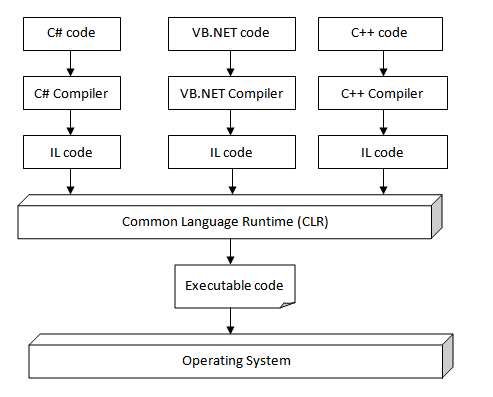
\includegraphics[width=\linewidth]{./images/clrArchitecture.png}
	\end{center}
	\caption{Common Language Runtime : Architecture \cite{clrarchitecure}}
	\label{fig:clrarchitecture}
\end{figure}

The Common Language Runtime (CLR) is virtual component of Microsoft's .net framework. It provides runtime environment which runs the code from various languages and also provides environment which makes software development process very easy \cite{Kennedy:2001:DIG:381694.378797}. Figure \ref{fig:clrarchitecture} shows architecture of CLR.

Tools and compilers expose CLR's functionality, so that you can take advantage of this common language runtime's managed execution environment. The code written to target common language runtime is known as managed code. This code can be benefited from features such as cross-language integration, cross-language exception handling, versioning, and security by providing simplied way for component interactions \cite{commonlanguageruntime}.


Compilers and tools able to produce the output consumed by the common langauge runtime, because, format of metadata, type systems are defined by the public standard called the ECMA Common Language Infrastructure \cite{Gough:2001:CNC:559569}.

Compiler emits metadata describing members, types, and references in your managed code to insure common language runtime provides services to managed code. This metadata is used to load and locate classes, load instances in memory, generate nastive code, enforce security \cite{Gough:2001:CNC:559569}.

Achieving even slight levels of language interoperability is pretty difficult because the wide variation in programming language features, and implementations. The CLR makes it easy to build components, and application whose objects can interact with each other across the languages. Code written in different languages can be integrated, their behavior is tightly integrated. For example, class written in one language can be derived from the class written in other language and can call method of the class it is derived from. We can also pass instance of the class (Object) from one language to another. This is possible because language compilers, and tools uses common type system provided by CLR and they follow the CLR’s standard rule for defining, creating, and pertaining types \cite{Kennedy:2001:DIG:381694.378797}.


CLR provides following benefits: 

1) Language inter-operation ability.

2) Performance enhancements.

3) Garbage Collection.

4) Support for exception handling.



\subsection{JVM}

// Add JVM related stuff after asking professor.

\cite{Singer:2003:JVC:957289.957341} discusses about difference between JVM and CLR.

\section{Java Scripting APIs}

After Java 6, java supports incorporating code written in scripting languages directly into Java. It enables developers to access their code written in scripting language directly into Java applications. It began new generation of multi-language application called as polyglot applications (where java language can work together with other scripting languages). \cite{Juneau2017}

With Java 6, developers were able to construct java applications containing scripts developed in languages like Java Script, and Python. It uses javaScript engine called Rhino in Java 6.  It is an implementation of the JavaScript engine, built entirely in Java. It contains full support for JavaScript, but it might not support some new javaScript standard as it is based on older javaScript Engine \cite{Juneau2017}.


In Java 6, this scripting functionality is provided by javax.script package. The package contains very simple and small APIs for accessing javaScripts. Scripting APIs are accessible through scriptEngineManager class. scriptEngineManager objects can search for script engines by means of jar file service detection mechanism.

According to Java documentation \cite{javascripting} Way to access nashorn engine in Java:

1.	Import the javax.script package.

2.	Create a ScriptEngineManager object.

JavaScripting APIs can be accessed through the ScriptEngineManager class. A ScriptEngineManager object is used to instantiate ScriptEngine objects and maintain global variable values shared by API. 

3.	Obtain instance of ScriptEngine from the manager with getEngineByName() method.

getEngineByName() method takes one string parameter with name of the script engine. To obtain instance of nashorn engine pass “nashorn”. We can also use one of the following arguments "ecmascript", "ECMAScript", "Nashorn", "JavaScript", "javascript", "js", "JS".
 
After, we have Nashorn engine instance, we can use to embed scripts in our Java application. Let's see some of the examples which shows the use of nashorn.

\textbf{Example 1 - Evaluating a statement}


Following code shows example which can evaluate "Hello world !" using Nashorn.


\begin{lstlisting}[frame=single]
import javax.script.*;

public class EvaluateScript {
 public static void main(String[] args) throws Exception {
  ScriptEngineManager manager = new ScriptEngineManager();
  ScriptEngine engine = manager.getEngineByName("nashorn");
  
  // evaluate JavaScript code
  engine.eval("print('Hello, World')");
 }
}
\end{lstlisting}

In the example shown above, script engine calls the eval() method and executes javaScript string passes as an argument to eval() function. 


\textbf{Example 2 - Evaluating a Script File}

\begin{lstlisting}[frame=single]
import javax.script.*;

public class EvalFile {
 public static void main(String[] args) throws Exception {
  ScriptEngineManager manager = new ScriptEngineManager();
  ScriptEngine engine = manager.getEngineByName("nashorn");
  
  engine.eval(new java.io.FileReader("script.js"));
 }
}
\end{lstlisting}

In the example shown in above, eval() method uses fileReader that reads Java Script file and evaluates it.


\textbf{Example 3 - Exposing a Java Object as a Global Variable}

\begin{lstlisting}[frame=single]
import javax.script.*;
import java.io.*;

public class ScriptVars {
 public static void main(String[] args) throws Exception {
  ScriptEngineManager manager = new ScriptEngineManager();
  ScriptEngine engine = manager.getEngineByName("nashorn");
  
  // create File object
  File f = new File("test.txt");
  
  // expose File object as a global variable to the engine
  engine.put("file", f);
  
  // evaluate JavaScript code and access the variable
  engine.eval("print(file.getAbsolutePath())");
 }
}

\end{lstlisting}

In the example shown above, file object created in Java is exposed to the nashorn engine as a global variable as the name file using put() method. Eval() function then calls javascript code which access this variable as global variable, and calls getAbsolutePath() method.